% State of research
\chapter{Hauptteil}

\section{Link}
Das ist ein \hyperref[ch:intro]{Link}.

\section{Liste}
\begin{itemize}
    \item \textbf{Unzureichendes Wissen:} Studenten sind besonders zu Beginn ihres Studiums nicht mit wissenschaftlicher Methodik vertraut und kennen \ggf{} nicht die Regeln zum korrekten Zitieren oder Referenzieren.
    \item \textbf{Effizienzsteigerung:} Durch Aneignung fremder Leistungen wird der eigene Arbeitsaufwand reduziert und bessere Ergebnisse können in kürzerer Zeit erzielt werden.
    \item \textbf{Einstellung zur Aufgabe:} Vereinzelt fehlt das Verständnis für die Bedeutsamkeit der Aufgabenstellung. Dies kann in manchen Fällen auf ein fehlendes Vertrauen in die Lehrperson zurückgeführt werden.
\end{itemize}

\section{Aufzählung}
\begin{enumerate}[label=RQ\arabic*.]
    \item Was wird in der Wissenschaft als Plagiat bezeichnet?
    \item Welche Möglichkeiten gibt es, um Plagiate zu vermeiden, erkennen und angemessen zu ahnden?
    \item Welche frei verfügbaren Tools eignen sich für die CaPD?
    \item Wo besteht noch Verbesserungspotential?
\end{enumerate}

\section{Gegliederte Beschreibung}
\begin{description}[style=unboxed, leftmargin=0cm]
    \item[Ein Beispiel] Sei Plagiatsfall \(s=s_{plg}\cup s_{src}=\{(1,d_{plg}),(2,d_{plg}),(3,d_{plg})\}\cup\{(4,d_{src}),(5,d_{src}),(6,d_{src}),(7,d_{src})\}\), der durch die Plagiatserkennungen \(r_1=(r_1)_{plg}\cup (r_1)_{src}=\{(1,d_{plg})\}\cup\{(4,d_{src}),(5,d_{src})\}\) und \(r_2=(r_2)_{plg}\cup (r_2)_{src}=\{(3,d_{plg}),(4,d_{plg})\}\cup\{(7,d_{src})\}\) teilweise erkannt wird.\footnote{Es mag zunächst ungewöhnlich erscheinen, dass \(|s_{plg}|<|s_{src}|\) oder \((4,d_{plg})\notin s_{plg}\), aber \((4,d_{plg})\in(r_2)_{plg}\). Diese Fälle sind jedoch keineswegs Ausnahmen. Besonders bei semantischen Plagiaten haben Plagiat- und Quelltextfragmente in der Praxis nur selten dieselbe Länge und es kommt vermehrt zu falsch positiven Ergebnissen.}
    In diesem einfachen Beispiel existiert nur ein Plagiatsfall und zwei zugehörige Plagiatserkennungen.
    Folglich ist \(|S|=|\{s\}|=1\) und \(|R|=|\{r_1,r_2\}|=2\).
    \item[Bestimmung der Genauigkeit] Für die Genauigkeit \(\prc_{macro}(S,R)\) muss nun für jede Erkennung \(r\in R\) der Wert des Bruchs \(\frac{|\bigcup_{s\in S}(s\sqcap r)|}{|r|}\) bestimmt werden.
    Sowohl \(r_1\) als auch \(r_2\) erkennen (einen Teil von) \(s\), daher gilt für beide \(s\sqcap r=s\cap r\).
    Beide Plagiatserkennungen sind gleich mächtig mit \(|r_1|=|r_2|=3\), was sich aus ihren Definitionen einfach abzählen lässt.
    Es verbleibt also nur noch die Berechnung der Kardinalität der Schnittmengen aus den Plagiatserkennungen und dem Plagiatsfall \(s\).
    Für \(r_1\) ergibt sich hier \(|s\cap r_1|=|r_1|=3\), da die Plagiatserkennung keine falsch positiven (plagiierten) Zeichen zurückgibt.
    Bei \(r_2\) sieht das anders aus, \(|r_2|>|s\cap r_2|=|\{(3,d_{plg})\}\cup\{(7,d_{src})\}|=2\).
\end{description}

\section{Tabelle}
\cref{tab:coverage} skizziert seine wesentlichen Ideen.
% Please add the following required packages to your document preamble:
% \usepackage{booktabs}
% \usepackage{multirow}
% \usepackage{graphicx}
% \usepackage[table,xcdraw]{xcolor}
% If you use beamer only pass "xcolor=table" option, i.e. \documentclass[xcolor=table]{beamer}
% \usepackage[normalem]{ulem}
% \useunder{\uline}{\ul}{}
% \usepackage{lscape}
\begin{landscape}
  \begin{table}
  \centering
  \resizebox{\textheight}{!}{%
  \begin{tabular}{@{}
  >{\columncolor[HTML]{C0C0C0}}l |l|l|l|l|l|l|ll@{}}
  \cellcolor[HTML]{9B9B9B}{\color[HTML]{9B9B9B} } &
    \multicolumn{2}{c|}{\cellcolor[HTML]{C0C0C0}{\ul \textbf{Lexikalische Erkennung}}} &
    \multicolumn{2}{c|}{\cellcolor[HTML]{C0C0C0}{\ul \textbf{Syntaktische Erkennung}}} &
    \multicolumn{2}{c|}{\cellcolor[HTML]{C0C0C0}{\ul \textbf{Semantische Erkennung}}} &
    \multicolumn{2}{c}{\cellcolor[HTML]{C0C0C0}{\ul \textbf{Gesamt}}} \\
  \multirow{-2}{*}{\cellcolor[HTML]{9B9B9B}{\color[HTML]{9B9B9B} }} &
    \multicolumn{1}{c|}{\cellcolor[HTML]{C0C0C0}\textbf{\(\bm{cov(S_{lex})}\)}} &
    \multicolumn{1}{c|}{\cellcolor[HTML]{C0C0C0}\textbf{Punkte}} &
    \multicolumn{1}{c|}{\cellcolor[HTML]{C0C0C0}\textbf{\(\bm{cov(S_{syn})}\)}} &
    \multicolumn{1}{c|}{\cellcolor[HTML]{C0C0C0}\textbf{Punkte}} &
    \multicolumn{1}{c|}{\cellcolor[HTML]{C0C0C0}\textbf{\(\bm{cov(S_{sem})}\)}} &
    \multicolumn{1}{c|}{\cellcolor[HTML]{C0C0C0}\textbf{Punkte}} &
    \multicolumn{1}{c|}{\cellcolor[HTML]{C0C0C0}\textbf{\(\bm{cov(S_{ges})}\)}} &
    \multicolumn{1}{c}{\cellcolor[HTML]{C0C0C0}\textbf{Punkte}} \\ \midrule
  \textbf{Ferret} &
    \(\frac{140}{154}\approx 91\% \) &
    3 &
    \(\frac{120}{164}\approx 73\%\) &
    2 &
    \(\frac{61}{169}\approx 36\%\) &
    1 &
    \multicolumn{1}{l|}{\(\frac{321}{487}\approx 66\%\)} &
    2 \\ \midrule
  \textbf{JPlag} &
    \(\frac{116}{154}\approx 75\%\) &
    2 &
    \(\frac{104}{164}\approx 63\%\) &
    2 &
    \(\frac{31}{169}\approx 18\%\) &
    0 &
    \multicolumn{1}{l|}{\(\frac{251}{487}\approx 52\%\)} &
    2 \\ \midrule
  \textbf{plagiarism\_detection} &
    n/a &
    n/a &
    n/a &
    n/a &
    n/a &
    n/a &
    \multicolumn{1}{l|}{n/a} &
    n/a \\ \midrule
  \textbf{PlagZap} &
    \(\frac{95}{154}\approx 62\%\) &
    2 &
    \(\frac{49}{164}\approx 30\%\) &
    1 &
    \(\frac{25}{169}\approx 15\%\) &
    0 &
    \multicolumn{1}{l|}{\(\frac{169}{487}\approx 35\%\)} &
    1 \\ \midrule
  \textbf{\begin{tabular}[c]{@{}l@{}}Sanchez-Perez \etal{}\\ (PAN 2015)\end{tabular}} &
    \(\frac{154}{154}=100\%\) &
    3 &
    \(\frac{158}{164}\approx 96\%\) &
    3 &
    \(\frac{111}{169}\approx 66\%\) &
    2 &
    \multicolumn{1}{l|}{\(\frac{423}{487}\approx 87\%\)} &
    3 \\ \midrule
  \textbf{Sherlock} &
    \(\frac{117}{154}\approx 76\%\) &
    3 &
    \(\frac{158}{164}\approx 96\%\) &
    3 &
    \(\frac{114}{169}\approx 67\%\) &
    2 &
    \multicolumn{1}{l|}{\(\frac{389}{487}\approx 80\%\)} &
    3 \\ \midrule
  \textbf{SIM} &
    \(\frac{55}{154}\approx 36\%\) &
    1 &
    \(\frac{31}{164}\approx 19\%\) &
    0 &
    \(\frac{29}{169}\approx 17\%\) &
    0 &
    \multicolumn{1}{l|}{\(\frac{115}{487}\approx 24\%\)} &
    0 \\ \midrule
  \textbf{text-matcher} &
    \(\frac{116}{154}\approx 75\%\) &
    2 &
    \(\frac{77}{164}\approx 47\%\) &
    1 &
    \(\frac{12}{169}\approx 7\%\) &
    0 &
    \multicolumn{1}{l|}{\(\frac{205}{487}\approx 42\%\)} &
    1 \\ \midrule
  \textbf{WCopyfind} &
    \(\frac{135}{154}\approx 88\%\) &
    3 &
    \(\frac{110}{164}\approx 67\%\) &
    2 &
    \(\frac{46}{169}\approx 27\%\) &
    1 &
    \multicolumn{1}{l|}{\(\frac{291}{487}\approx 60\%\)} &
    2
  \end{tabular}%
  }
  \caption{Vergleich der wortbasierten Plagiatsfallüberdeckung und Einordnung auf Punkteskala}\label{tab:coverage}
  \end{table}
  \end{landscape}

\section{Bild}
\begin{figure}
    \centering
    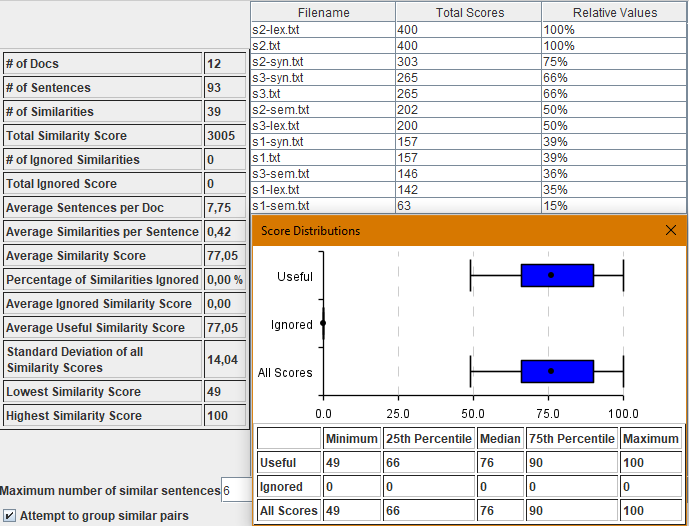
\includegraphics[width=0.9\textwidth]{sherlock-overview}
    \caption{Ergebnisübersicht von \emph{Sherlock}}\label{fig:sherlockSum}
\end{figure}

\section{Tikz}
\begin{figure}
    \centering
    \resizebox{0.9\textwidth}{!}{%
        \begin{tikzpicture}[grow=right, level distance=4cm, sibling distance=0.5cm]
            \Tree [.Plagiat
                    [.{andere Plagiate} {Plagiat mit Erlaubnis} Selbstplagiat Ghostwriting ]
                    [.intelligent
                            [.ideenbasiert Struktur\-plagiat ]
                            [.semantisch {Übersetzungs\-plagiat} {unzulässiges Paraphrasieren} ]
                    ]
                    [.{buchstäblich/\\wörtlich}
                            [.syntaktisch {Synonym\-substitution} {technische Verschleierung} ]
                            [.lexikalisch {schein\-paraphrasieren} {wörtliches Kopieren} ]
                    ]
            ]
        \end{tikzpicture}
    }%
    \caption{Plagiat -- Eine Taxonomie}\label{fig:taxonomy}% chktex 8
\end{figure}

\section{Textzitat}
So definiert der Duden Plagiat als \textcquote{Dudenredaktion.2018}{unrechtmäßige Aneignung von Gedanken, Ideen \oae{} eines anderen auf künstlerischem oder wissenschaftlichem Gebiet und ihre Veröffentlichung; Diebstahl geistigen Eigentums}.

\section{Blockzitat}
\begin{displaycquote}[1]{Manning.2018cop.2008}
    Information retrieval (IR) is finding material (usually documents) of an unstructured nature (usually text) that satisfies an information need from within large collections (usually stored on computers).
\end{displaycquote}

\section{Indirektes Zitat}
Außerdem entsteht -- insbesondere bei studentischen Arbeiten -- zumeist kein messbarer Verlust für den Autor, während dies bei einem Diebstahl sehr wohl der Fall wäre \indcite[2\psq]{TeddiFishman.2009}.

\section{Gleichung}
\begin{equation}\label{eqn:prec}
    \mbox{prec}=\frac{|\{\mbox{relevant results}\}|}{|\{\mbox{results}\}|}
\end{equation}

\section{Listing}
\begin{listing}
    \inputminted{bat}{lst/ferret.txt}
    \caption{Konsolenausgabe von \emph{Ferret}}\label{lst:ferret}
\end{listing}

\section{Langes Listing}
\begin{longlisting}
    \inputminted{xml}{lst/ferret.xml}
    \caption{Detaillierter Bericht von \emph{Ferret}}\label{lst:ferretXml}
\end{longlisting}